\documentclass[10pt,twocolumn,letterpaper]{article}

\usepackage{diagbox}
\usepackage{statcourse}
\usepackage{times}
\usepackage{epsfig}
\usepackage{graphicx}
\usepackage{amsmath}
\usepackage{amssymb}
\usepackage{courier}
\usepackage{caption}
\usepackage{subfigure}
% Include other packages here, before hyperref.

% If you comment hyperref and then uncomment it, you should delete
% egpaper.aux before re-running latex.  (Or just hit 'q' on the first latex
% run, let it finish, and you should be clear).
\usepackage[breaklinks=true,bookmarks=false]{hyperref}


\statcoursefinalcopy


\setcounter{page}{1}
\begin{document}


%%%%%%%%%%%%%%%%%%%%%%%%%%%%%%%%%%%%%%%%%%%%%%%%%%%%%%%%%%%%%%%
% DO NOT EDIT ANYTHING ABOVE THIS LINE
% EXCEPT IF YOU LIKE TO USE ADDITIONAL PACKAGES
%%%%%%%%%%%%%%%%%%%%%%%%%%%%%%%%%%%%%%%%%%%%%%%%%%%%%%%%%%%%%%%



%%%%%%%%% TITLE
\title{DeepFake Usage Detection Using Neural Network\\

\begin{small}
See code at:\url{https://github.com/nemowch905/stat453project}
\end{small}}

\author{Chong Wei\\
{\tt\small cwei48@wisc.edu}
\and
Youhui Ye\\
{\tt\small yye65@wisc.edu}
\and
Fangyang Chen\\
{\tt\small fchen92@wisc.edu}
}

\maketitle
%\thispagestyle{empty}



% MAIN ARTICLE GOES BELOW
%%%%%%%%%%%%%%%%%%%%%%%%%%%%%%%%%%%%%%%%%%%%%%%%%%%%%%%%%%%%%%%


%%%%%%%%% ABSTRACT
\begin{abstract}
DeepFake is a popular neural network application in video editing, which transfers people's faces to others. Thus we aim to develop a method that can detect DeepFake usage in a video set provided by kaggle.com to see if a video is edited or not. We used a Histogram of Oriented Gradients method provided by package \texttt{dlib} in data processing to extract frontal face features from video screenshots, with data augmentation to reduce overfitting. And a convolution neural network structure Xception is conducted by \texttt{PyTorch} to perform classification. The network is constructed on Google Colab for GPU access. The result in the test set turns out to be 81.48\%, after 200 epochs' training. There remain problems in accuracy optimization and FPR bias due to small data size and simple function calls, but the result is effective enough to show the validity of the method. It is a rather inspiring and systematic workflow engaging all detailed steps in the CNN classification problem with a satisfying result.
\end{abstract}

%%%%%%%%% BODY TEXT
\section{Introduction}

DeepFake is a currently popular technique that allows people's faces to be replaced by other people's in images or videos. As a media of message transportation, vision editing will cause a distortion of information in many ways, no matter what the original intentions are. It may lead to reputation damage or wrong judicial judgement by defamation. Also, it may leads to twisted propaganda caused by politicians.

This technique is realized by neural network consists of an encoder and a decoder. Encoder transports an image into a lower latent space which contains key features including face characteristics and movements. And a decoder reconstructs the latent space back into an image with a model that is specifically trained for a target. 

Then the topic comes up naturally. We tried to fight against DeepFake abuse using convolutional neural network to identify if a video is being edited by DeepFake. This will help people determine what to believe without doing harm to the technology industry.

More specifically in methodology, in data preprocessing part, \texttt{dlib} package is used to detect and process image files screenshot from video data set.  Regarding to network structure, we refer to a essay introducing Xception, which is an variant of Inception architecture. With this network structure, we could construct and conduct models on training video sets.

\section{Related Work}
\subsection{Data Preprocessing}

To transfer videos into available data type, we used \texttt{dlib} to process screenshots. It uses a method called Histogram of Oriented Gradients and Linear Support Vector Machines Object Detection (roughly referred as HoG). It's firstly introduced in 2005 by Navneet Dalal and Bill Triggs\cite{dalal2005histograms}. Compared to Haar cascade classifiers provided by OpenCV, it doesn't require tedious parameter tuning in \texttt{cv2.detectMultiScale}. It's also more accurate and helps you struggle less in balancing False Positive Rate by more than an order of magnitude relative to the best Haar wavelet based detector.\cite{mohan2001example}

\begin{figure}[t]
    \centering
    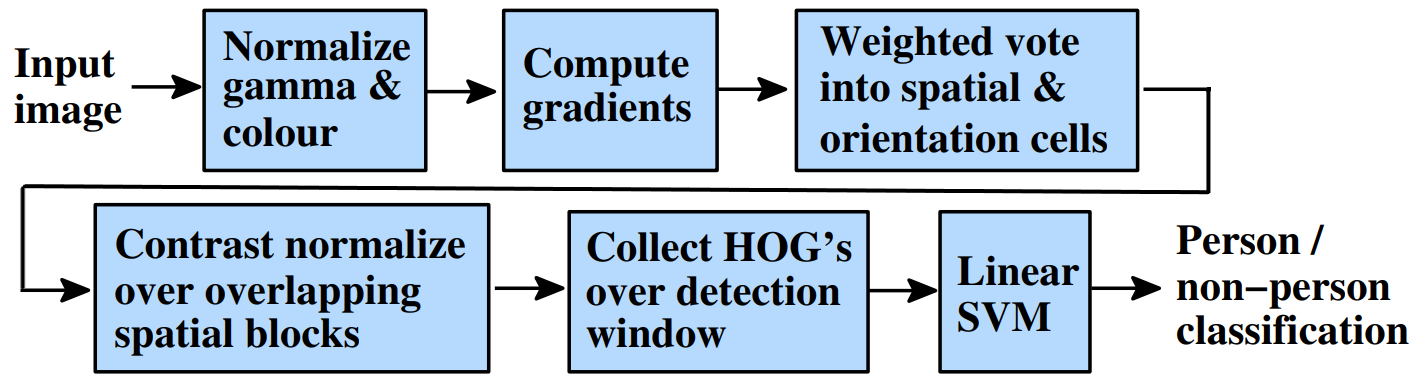
\includegraphics[width=0.5\textwidth]{figures/HoG_flow.png}
    \caption{Histogram of Oriented Gradients Work Flow \cite{dalal2005histograms} }
\end{figure}

A stack of overlapping blocks make up the detector window and HOG features are extracted from it. Then it trains a linear SVM model to classify the feature vectors. The detection window runs all over the image at all positions and all scales.Then the conventional non-maximum suppression runs on the output pyramid to detect object instances. 


\subsection{Network}

\begin{figure*}
    \centering
    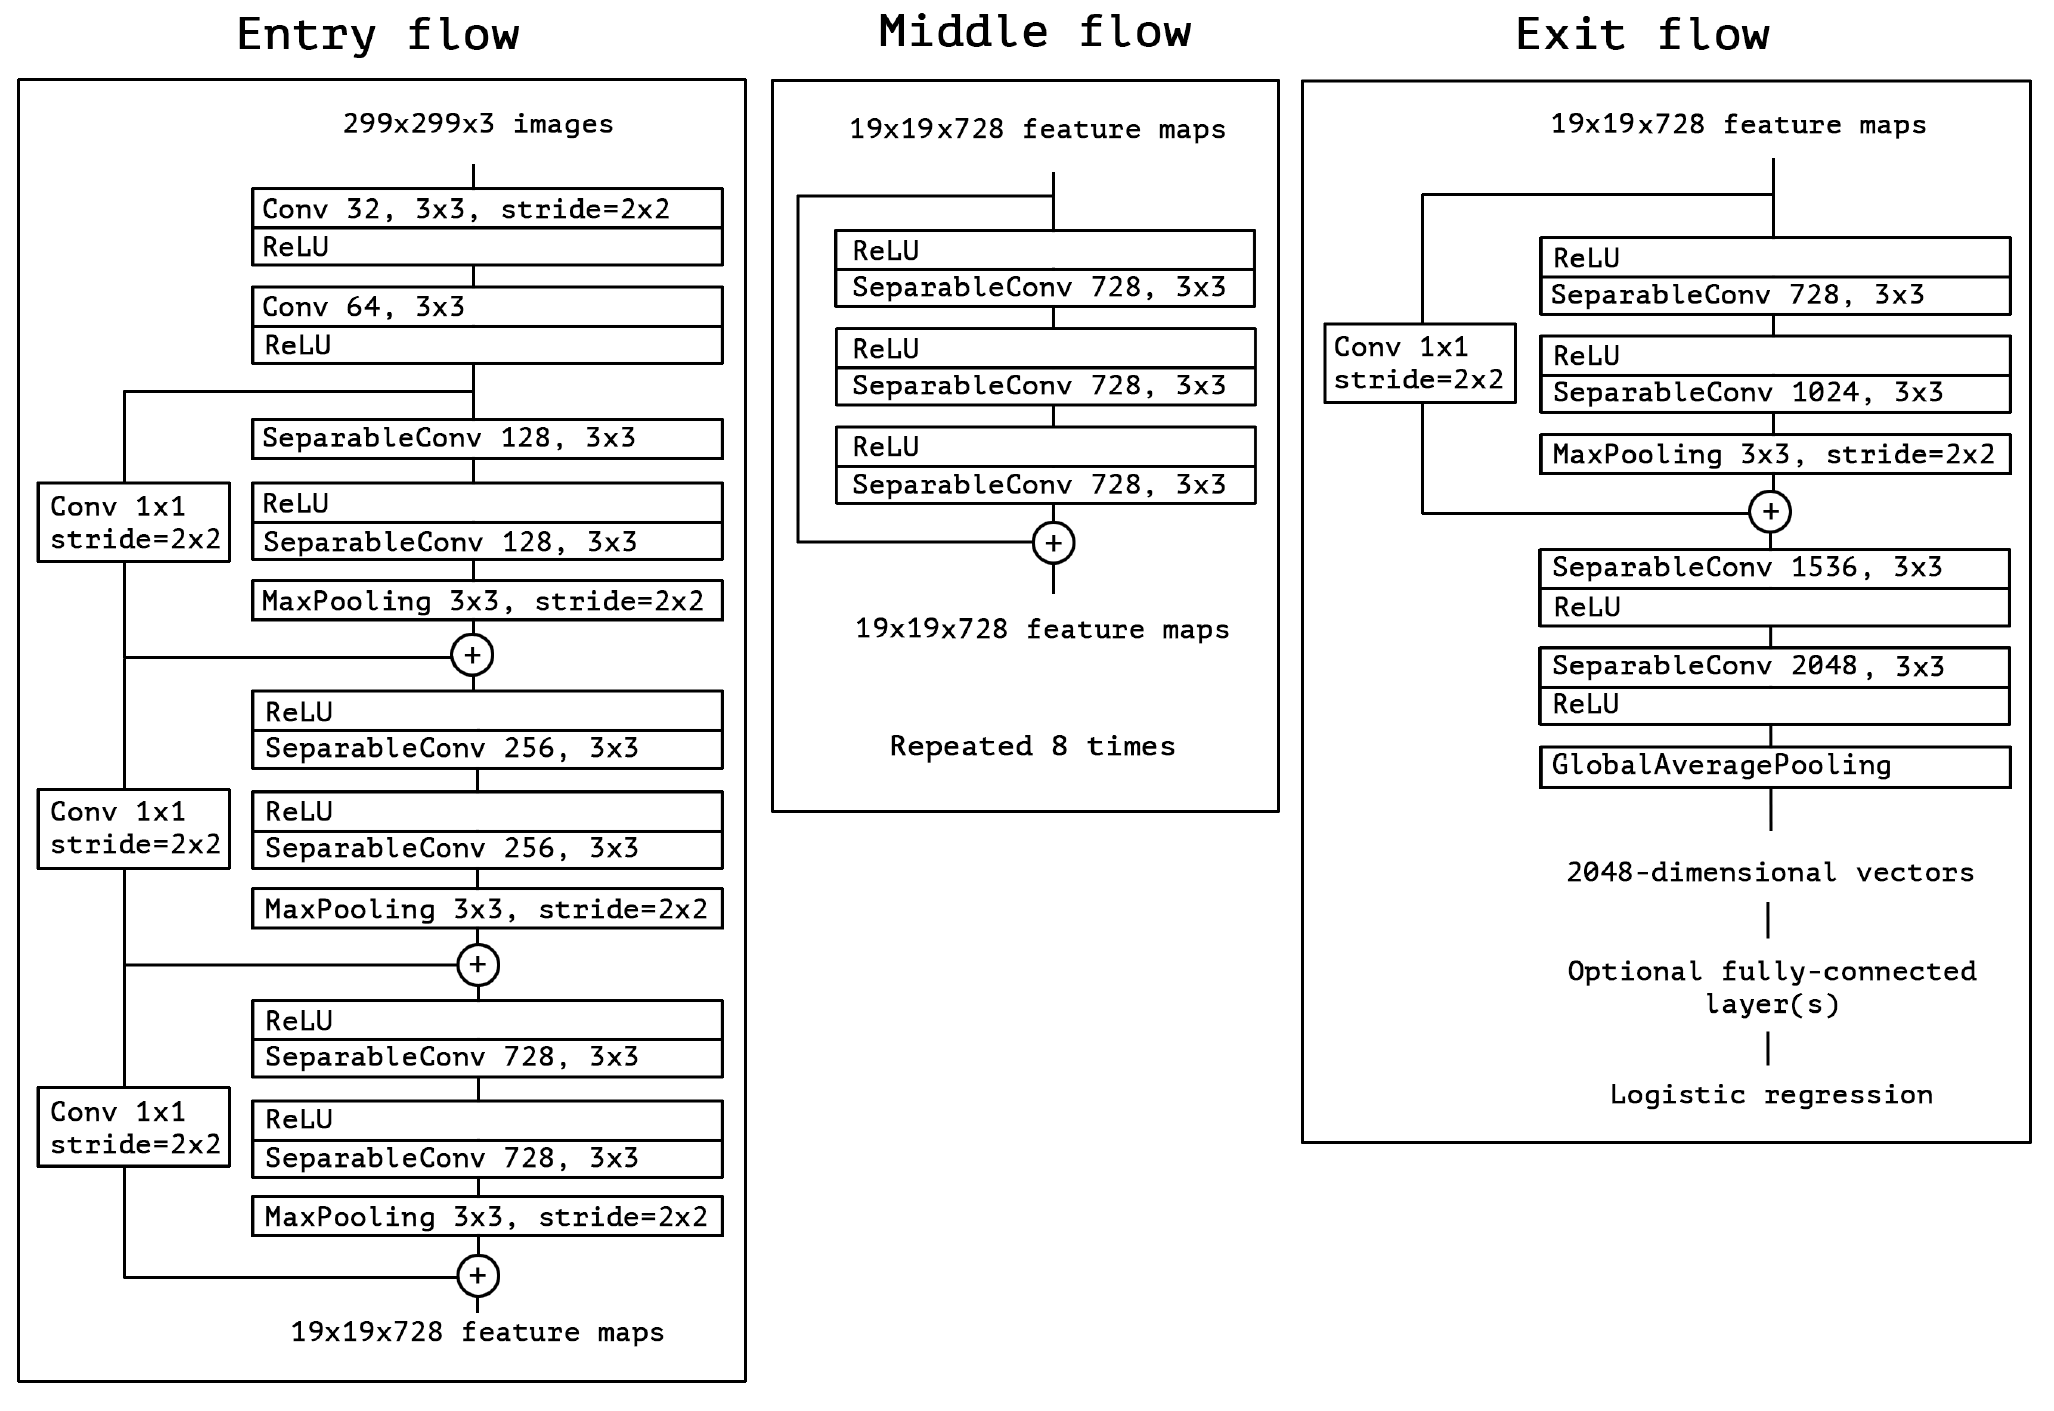
\includegraphics[width=\textwidth]{figures/figure1.png}
    \caption{Specific Xception Network Structure \cite{chollet2017xception} }
    \label{fig:2}
\end{figure*}

We mainly accepted the suggestion given by Andreas Rozssler and other coauthors(2019)\cite{rossler2019faceforensics++}. In the paper, they introduced there are 4 types of fake image generators, which are DeepFake, FaceSwap, Face2Face and NeuralTextures. The former 2 methods are facial replacement methods. They exploit the corresponding 3D geometry of both source and target face to realize the synthesis. The later 2 methods are based on facial reenctment, which combine both 3D model reconstruction and learning based method to generate their output. The authors applied several different convolutional neural networks to the fake images generated by those 4 ways. As a result, Xception Network with cropped images gives the best predictions. 

Our main network reference is Xception structure developed by Google.\cite{chollet2017xception} It's a enhancement of Inception architecture so it becomes the portmanteau of Extream and Inception. 

Inception architecture is introduced by Szegedy et al. 2014.\cite{Szegedy_2015_CVPR} It was inspired by the earlier architecture called Network-In-Network. Inception and it's following refined models have been the best performing models on the ImageNet dataset.

Inception method is first developed by using the global average pooling layer instead of the fully connected layer. The amount of parameters is greatly reduced, and the model is called Inception V1. In the following Inception V2\cite{DBLP:journals/corr/IoffeS15}, the Batch Normalization method was introduced to speed up the convergence of training. And in the Inception V3 \cite{szegedy2016rethinking} model, by splitting the two-dimensional convolutional layer into two one-dimensional convolutional layers, not only the number of parameters is reduced, but also eases overfitting.

Convolutional layers attempt to study filters in a 3-dimensional space with 2 spatial dimensions (width and height) and one channel dimension. Therefore, the task of a convolution kernel is to demonstrate the inter-channel and spatial correlation at the same time. The basic hypothesis of the Inception module is to make this process easier and more efficient by explicitly dividing it into a series of operations independent of cross-channel and spatial correlation.

The original hypothesis of Inception is that cross-channel correlations and spatial correlations are decoupled so we'd better not to map them jointly. But based on a stronger hypothesis, if we consider  the mapping of cross-channel and spatial correlation to feature space is entirely decoupled, then we have a more \textit{extreme} form of the architecture. Under this circumstance, the new extreme Inception module can be reformulated into a $1\times1$ convolution that would operate on the output channels, which the segments are not overlapping.

\begin{figure}[h]
\centering
\subfigure[Original Inception]{
\begin{minipage}{8cm}
\centering 
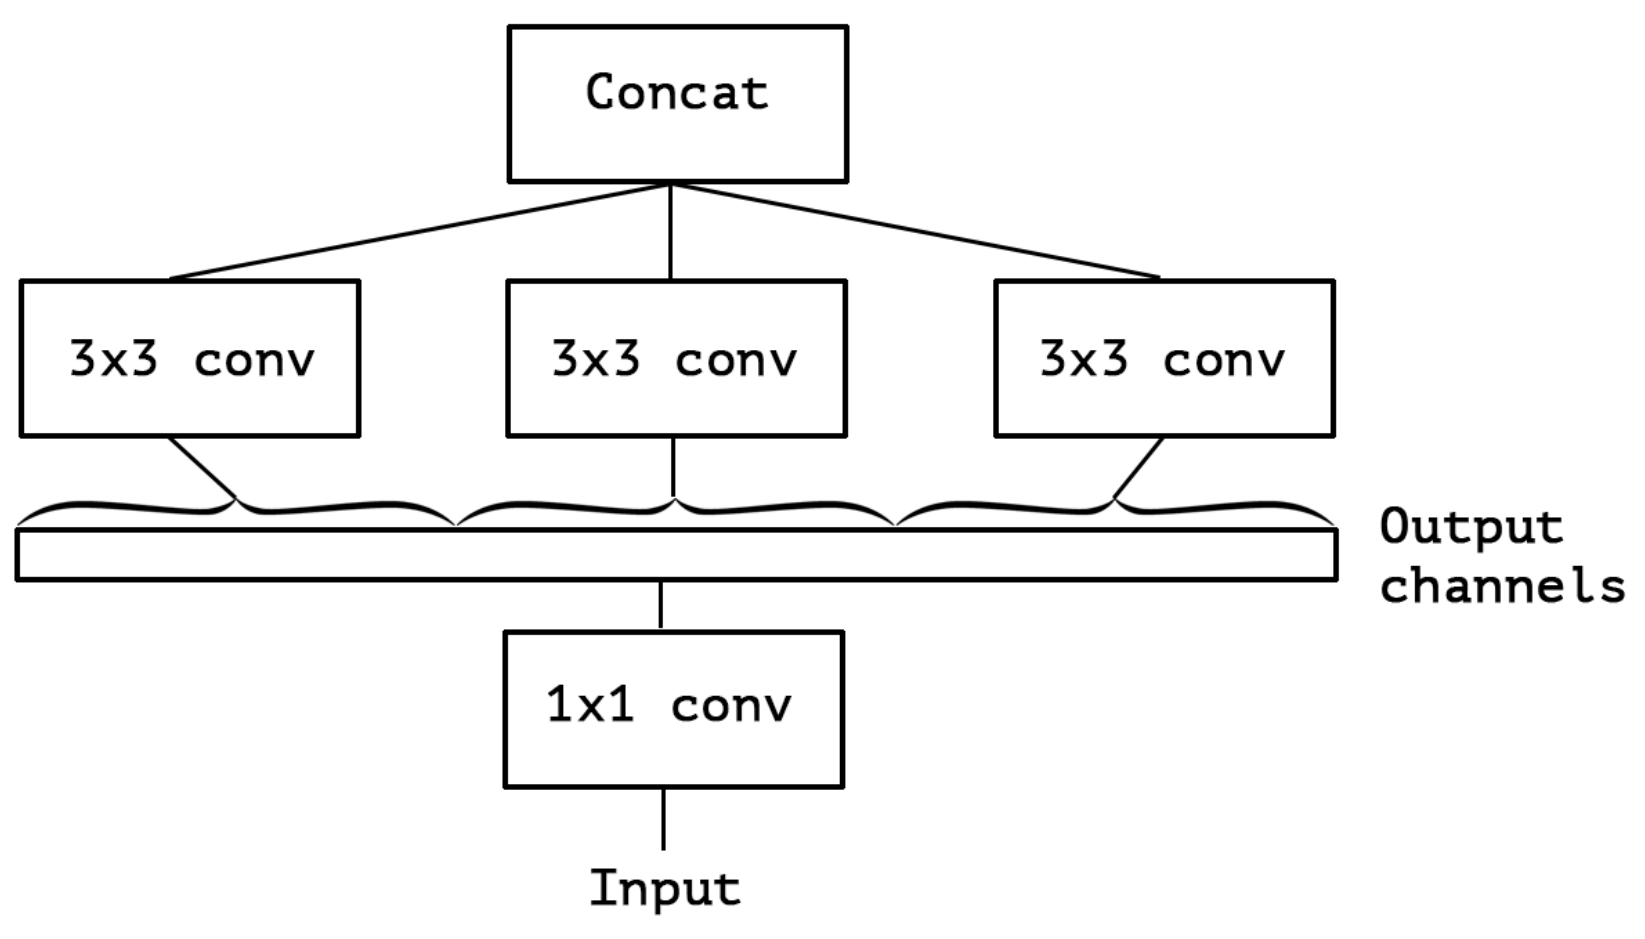
\includegraphics[width=\textwidth]{figures/inception.png} 
\end{minipage}
}
\subfigure[Extreme Inception]{ 
\begin{minipage}{8cm}
\centering
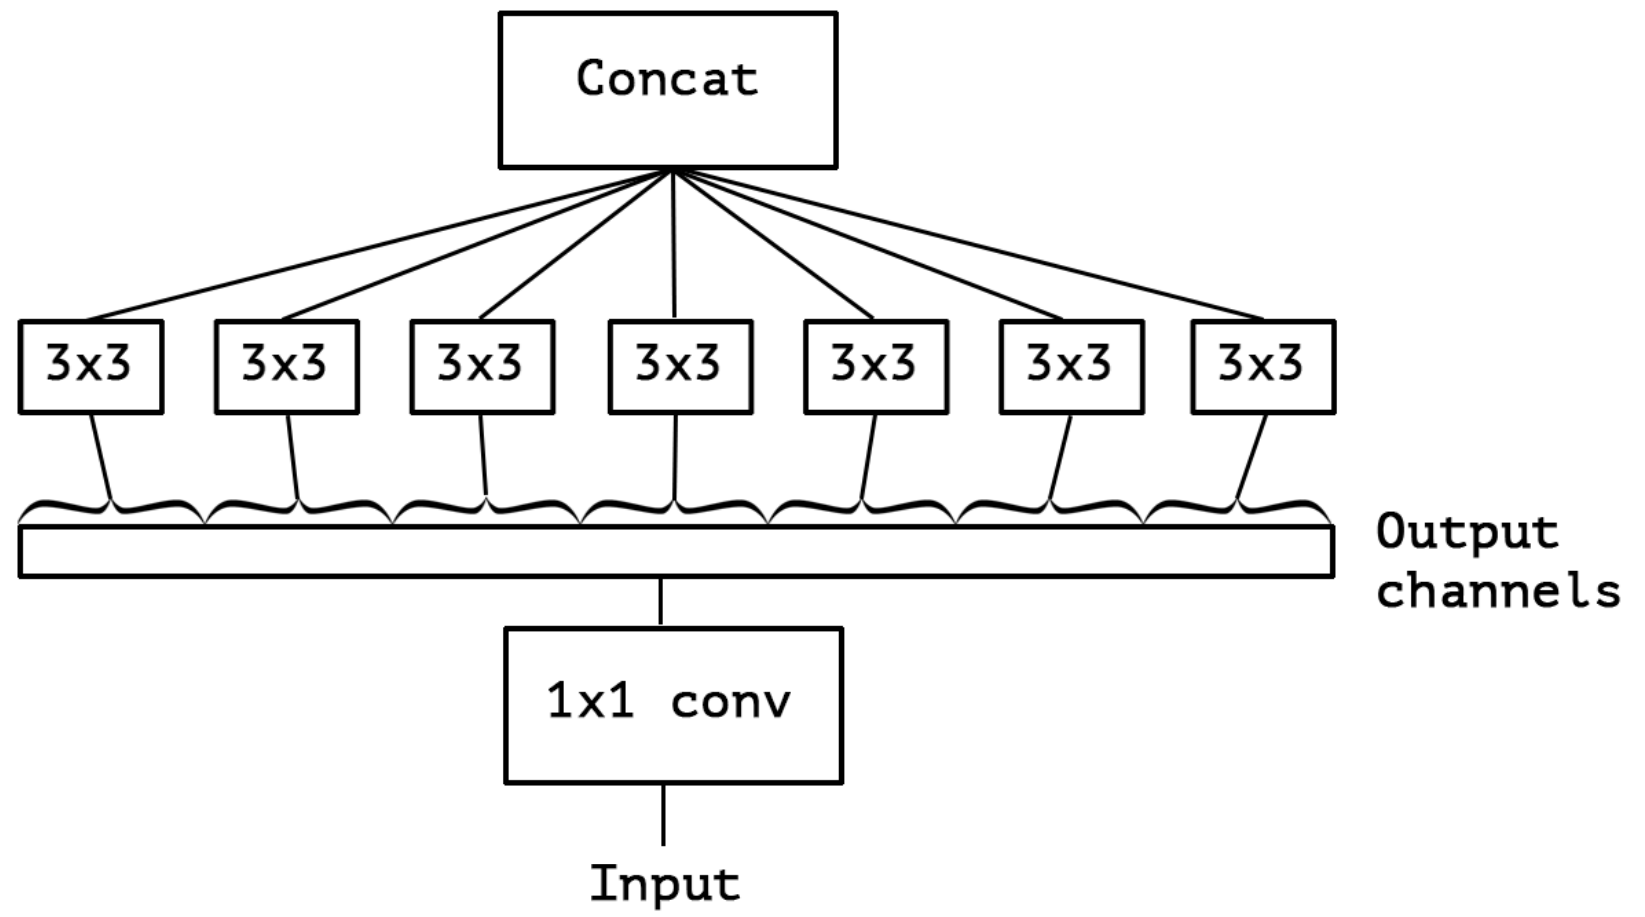
\includegraphics[width=\textwidth]{figures/xception.png} 
\end{minipage}
}
\caption{Extreme version of inception\cite{chollet2017xception} }
\label{fig:1} 
\end{figure}

A sketch structure comparison is shown in Figure 2.


\section{Proposed Method}

\subsection{Face Detection}
Firstly we convert the images from RGB color to grey using \texttt{cv2.cvtColor}, for better compatibility. Function \texttt{dlib.get\_frontal\_face\_detector} is used to crop the screenshots into $299\times 299$ \texttt{dataloader}-friendly input image.

\subsection{Network Structure}
The Xception architecture is constructed by 36 layers which form the feature extraction base of the network. They are structured into 14 modules, which other than the first and last modules, all of them have linear residual connections around them. All in all, Xception is a linear stack of depth-wise separable convolution layers with residual connections.\cite{chollet2017xception} The assumption makes the architecture easier and clearer in construction as well as modification.
The architecture of Xception is illustrated in Figure 3.

To achieve depth-wise separable convolution, we firstly build a class \texttt{SeparableConv2d} to resemble the original built-in \texttt{nn.Conv2d}. For the 12 blocks amid the total 14 blocks, set \texttt{kernal\_size} to 3 to assemble the layers. Use built-in \texttt{nn.BatchNorm2d} for batch normalization (which follows every \texttt{Conv} layer and  \texttt{SeparableConv} layer, though not demonstrated in the Figure) and \texttt{nn.MaxPool2d} for 2D max pooling over an input signal composed of several input planes, when \texttt{stride} is not 1. Then class \texttt{Xception} organizes the former blocks with extending number of filters which is specifically shown in Figure 3.


\section{Experiments}

The whole experiment process is based on the proposed method as stated above. Andreas Rossler and other authors coded the Xception architecture and published it on github: \url{https://github.com/ondyari/FaceForensics}. After choosing our own loss function and optimization methods, we completed the training and testing parts. Finally, our trained Xception Net can predict if a face is fake based on a 299*299 RGB image. 

\begin{figure}
\begin{center}
   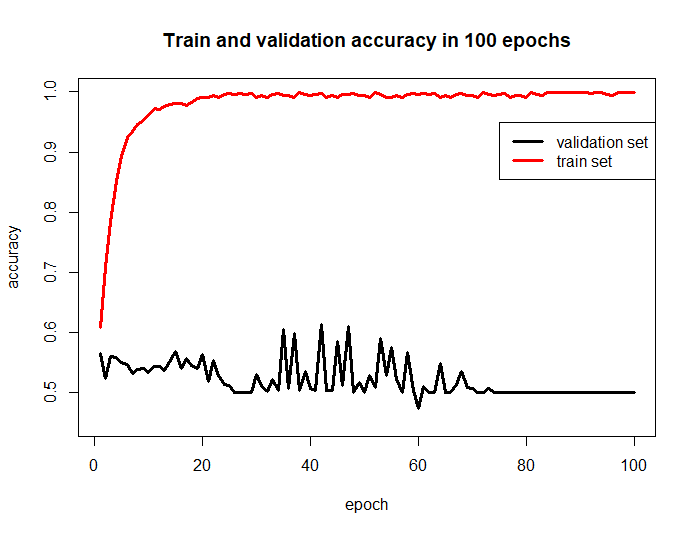
\includegraphics[width=\linewidth]{figures/Rplot04.png}
\end{center}
   \caption{Train and validation accuracy in 100 epochs}
\label{fig:google-scholar-2col}
\end{figure}

\subsection{Data Preprocessing} 

The original data set can be found on kaggle with the requirement of participating the DeepFake Detection Challenge \cite{kaggle.com}. The whole data set is of size bigger than 400 GB, containing 120,000 videos. There are 50 zip files on the website. This experiment was performed using part of it. 

We took screenshots on the videos every 80 frames and labeled them as real or fake by the corresponding videos. Then we cropped them with the 'get frontal face detector' function from dlib to get the face images. Since the ratio of real to fake is about 1:6, we used image augmentation to get more real samples. In this way, about 50000 images could be generated from one zip file. With google colab, the training time for 100,000 images is about 75 minutes per epoch(depends on which GPU is allocated). To accomplish the experiment on time, we decided to use only about 100,000 images for training.

\begin{figure}[h]
\centering
\subfigure[Fake(left):Real(right) Balance is 6:1]{
\begin{minipage}{8cm}
\centering 
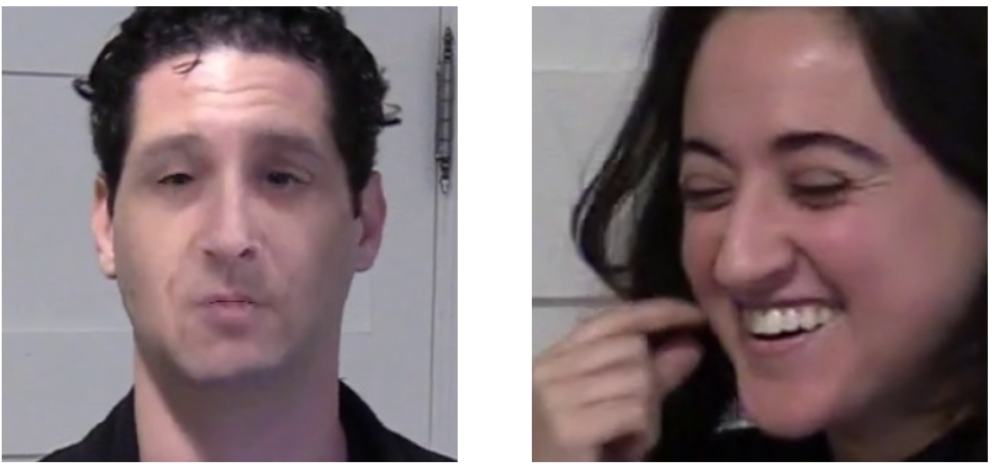
\includegraphics[width=\textwidth]{figures/balance.png} 
\end{minipage}
}
\subfigure[Augmentation]{ 
\begin{minipage}{8cm}
\centering
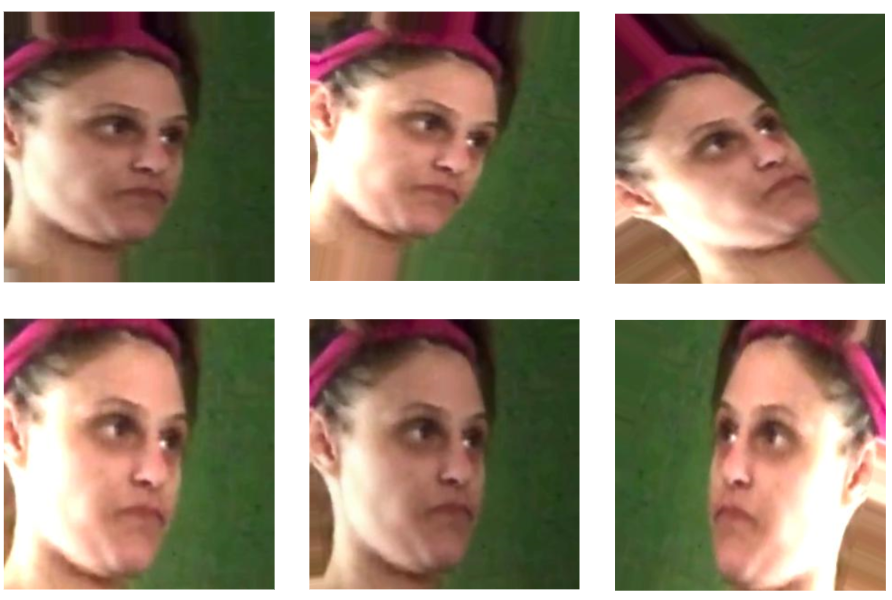
\includegraphics[width=\textwidth]{figures/augmentation.png} 
\end{minipage}
}
\caption{}
\end{figure}

We used 22.zip and 23.zip for training at first. There were 90501 images in train set. We chose 8000 images from 24.zip to avoid over-fitting problem. The results are not satisfying. Figure 3 shows the terrible over-fitting problem. The train set accuracy could reach 99\%, while the validation set kept to be 50\%. The model was predicting every image to be real. The problem was caused by train set. Though the train set is very large, all of the 90501 images are generated from only 2500 videos acted by less than 100 person.

So we enlarged the range. We used 14 zip packages (11.zip, 14.zip, 15.zip, 16.zip, 22.zip, 23.zip, 25.zip, 26.zip, 27.zip, 28.zip, 29.zip, 30.zip, 31.zip). Instead of adding real samples, we use subset of fake videos to solve the balance problem. For each package, we selected same amount of fake images as real images. We generated 93734 images as train set. And we used the same validation set for comparison. The train set\footnote{\url{https://drive.google.com/open?id=12PSpQAu2idM0Uyc82_0lNnU4e3GRt8aa}} and validation set\footnote{\url{https://drive.google.com/open?id=12aSIYkX6wfBg5Kdfvxj0G1-WS6qVQeRT}} are uploaded for downloading.

\subsection{Software}

Python 3.7 is the major language we used in this experiment. To be specific, 'dlib' was employed for face detection, 'cv2' was used in cropping images, and 'PyTorch' played a critical role in defining the Xception's architecture and training process. 

\subsection{Hardware}

The computer software mainly includes two parts. We conducted data preprocessing on each group member's lap-top, which are an i7 9th gen CPU + GTX1650 GPU, i5 8th gen CPU + Intel Iris Plus 655 GPU and an i5 8th gen CPU + Intel(R) UHD Graphics GPU. We finished data collecting and preprocessing on our laptops. Since the GPUs are not powerful enough, the primary work of training and testing were completed on the Google colaboratory. Colab pro provides Tesla T4 and P100. 

\subsection{Training} 

The training process is separated to several parts due to google colab connecting problem. We had to continue from checkpoint when the process was shut down because of disconnection. Google colab allocated GPU resource randomly. So the training process was based on both Tesla T4 and P100.

All of the images are normalized with the mean and standard deviation of the train set. The mean is (0.437900, 0.353218, 0.331976); the standard deviation is (0.242710, 0.234293, 0.232247). The number of total training epochs was 200. The batch size was 32. The number of workers was 2. The initial learning rate was 0.1 and reduced by 80\% every 50 epochs. We also used warm up training on the first epoch for better performance. We saved checkpoint every 5 epochs and saved the best accuracy model after 150 epochs.

\subsection{Testing} 

The test set videos are selected randomly from other zip packages (48.zip, 49.zip). It contains 486 videos. We took screenshots on the videos every 8 frames and cropped them to get the face images. Since some faces couldn't be detected by dlib, there were some ineffective images. Then we test the effective images' labels with our best model. We can get the probability that certain image's label is fake or real. The final probability of fake or real is calculated with following equation. The test set\footnote{\url{https://drive.google.com/open?id=1rVP-m72cNWcLn_kCGKpyccWpRAZZWIh3}} is uploaded for downloading.

$$P_{REAL}=\frac{1}{n}\sum_{i=1}^n R_i$$

$$P_{FAKE}=\frac{1}{n}\sum_{i=1}^n F_i$$

where 


\begin{itemize}

	\item n is the number of effective face images generated from certain video
	
	\item $R_i$ is the predicted probability of the image being REAL
	
	\item $F_i$ is the predicted probability of the image being FAKE

	
\end{itemize}

Then we compare $P_{REAL}$ and $P_{FAKE}$ to get the final label of certain video. Then we can get the accuracy on the whole test set.




\begin{figure}
\begin{center}
   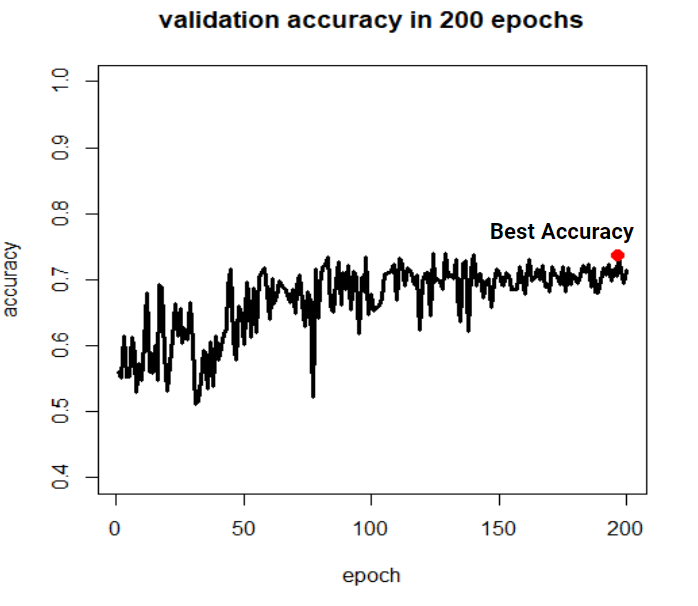
\includegraphics[width=\linewidth]{figures/plotval1.png}
\end{center}
   \caption{Validation accuracy in 200 epochs}
\label{fig:google-scholar-2col}
\end{figure}

\section{Results and Discussion}

\subsection{Results} 

The validation accuracy reached 73.58\% at 197th epoch as shown in figure 5. We saved the best model and used it for testing. The official test set is not available. The test set provided by kaggle is related to videos used for training. So we selected 486 videos randomly from videos we didn't use. The real task is to recognize if the video is real or not. Testing simply on face images is meaningless. Our test set contains 81 real videos and 405 fake videos. The accuracy is  81.48\%. 46 of real videos and 350 of fake videos are predicted correctly as shown in Table 1.

\begin{table}[h]
\centering
\caption{Test set result 1}
\begin{tabular}{|l|c|c|c|}
\hline
\diagbox{True}{Predicted} & Real & Fake & Total \\
\hline
Real & 46 & 35 & 81 \\
\hline
Fake & 55 & 350 & 405 \\   
\hline
Total & 101 & 385 & 486 \\ 
\hline
\end{tabular}
\end{table}

\begin{table}[h]
\centering
\caption{Test set result 2}
\begin{tabular}{|l|c|c|c|}
\hline
Precision & Recall & F1-score \\
\hline
0.9091 & 0.8642 & 0.8861 \\
\hline
\end{tabular}
\end{table}



\subsection{Discussion}

The precision and recall are 90.91\% and 86.42\% as shown in Table 2. So the model works well in detecting fake videos. The validation accuracy is not well enough. Actually, after 150 epochs, the accuracy kept floating at the range of 65\% to 75\%. It means the train set has been learned fully. And decreased learning rate didn't improve the model. The problem of over-fitting is not solved well enough.There are two reasons leading to the problem. 

The first one is about the face detecting process. Dlib is a mature package for face detecting. However, it has its limit.  Because accuracy face detecting function is too slow to deal with large amount of images, we used the simplest function, which performs badly on side face. It couldn't detect a face in about 20\% of the screenshots. And sometimes, it recognize other things shown in Figure 7 as faces. 

The second one is about the amount of images. We only used 1/3 of the data provided. More data would probably improve the performance.

\begin{figure}
\begin{center}
   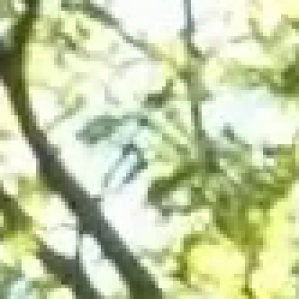
\includegraphics[width=0.5\linewidth]{figures/wrong img.jpg}
\end{center}
   \caption{A miss-detected face.}
\label{fig:google-scholar-2col}
\end{figure}



\section{Conclusions}

The initial goal was to build a model that could effectively detect fake videos. The results from our model are quite effective. Compared to past research and other competitor in deepfake detection challenge, the results are not good enough, as others work has performed noticeably better at times.

Our analysis was based on face image. There is some information missed during our experiment. The images are used separately. The abnormality from one frame to the next, which could be detected continually, is ignored. Considering the light factor, the background information may be useful as well. These could be future direction.

\section{Acknowledgements}

Our work was conducted for a class project and out of personal interest, and did not receive any funding from outside sources. Our professor, Sebastian Raschka, provided us with much of the foundational material for learning the deep learning techniques applied in this paper.

\section{Contributions}

\textbf{Project Report (writing)}

Introduction - Fangyang Chen

Related Work - Fangyang Chen, Youhui Ye

Proposed Method - Fangyang Chen, Youhui Ye

Experiments - Chong Wei, Youhui Ye

Results and Discussion - Chong Wei

Conclusions - Chong Wei

Contributions - Dan, Zheng Ni, Chong Wei\\

\textbf{Computational Tasks}

Preprocessing - Chong Wei, Fangyang Chen, Youhui Ye

Model building- Chong Wei, Fangyang Chen, Youhui Ye

Experiment - Chong Wei, Fangyang Chen

Result evaluating - Chong Wei, Youhui Ye



{
\bibliographystyle{ieee.bst}
\bibliography{bibliography.bib}
}

\end{document}
